\section{Experimental Apparatus}
\label{sec:experiment}

As discussed in \refS{subsec:prodproc}, the detection of \HToZg events requires
colliding protons head on at very high energies in order to produce a shower
of particles whose kinematic properties must be subsequently measured.
The first step, obtaining proton-proton collisions at high center-of-mass energies,
is accomplished by the accelerator complex that makes up the Large Hadron Collider.
Subsequently, the ATLAS detector takes up the difficult task of measuring
the proceeding shower of hadrons and leptons necessary to find the Higgs boson
as well as any new physics.
\refS{subsec:lhc} describes the LHC accelerator
complex in detail and \refS{subsec:atlas} provides an overview of the various
particle detection apparatus that make up the ATLAS detector.

\subsection{The Large Hadron Collider}
\label{subsec:lhc}
The Large Hadron Collider (LHC) is the world's largest and highest-energy particle
accelerator. The LHC sits in a circular tunnel 27 km in circumference under
the Franco-Swiss border near Geneva, Switzerland. The LHC accelerates protons
to a velocity of 99.9999964\% the speed of light \cite{LHCdesign}. The full
complex of accelerators that dump protons into the LHC and other CERN 
experiments is displayed in \refF{fig:accelerator}.

\begin{figure}
  \centering
  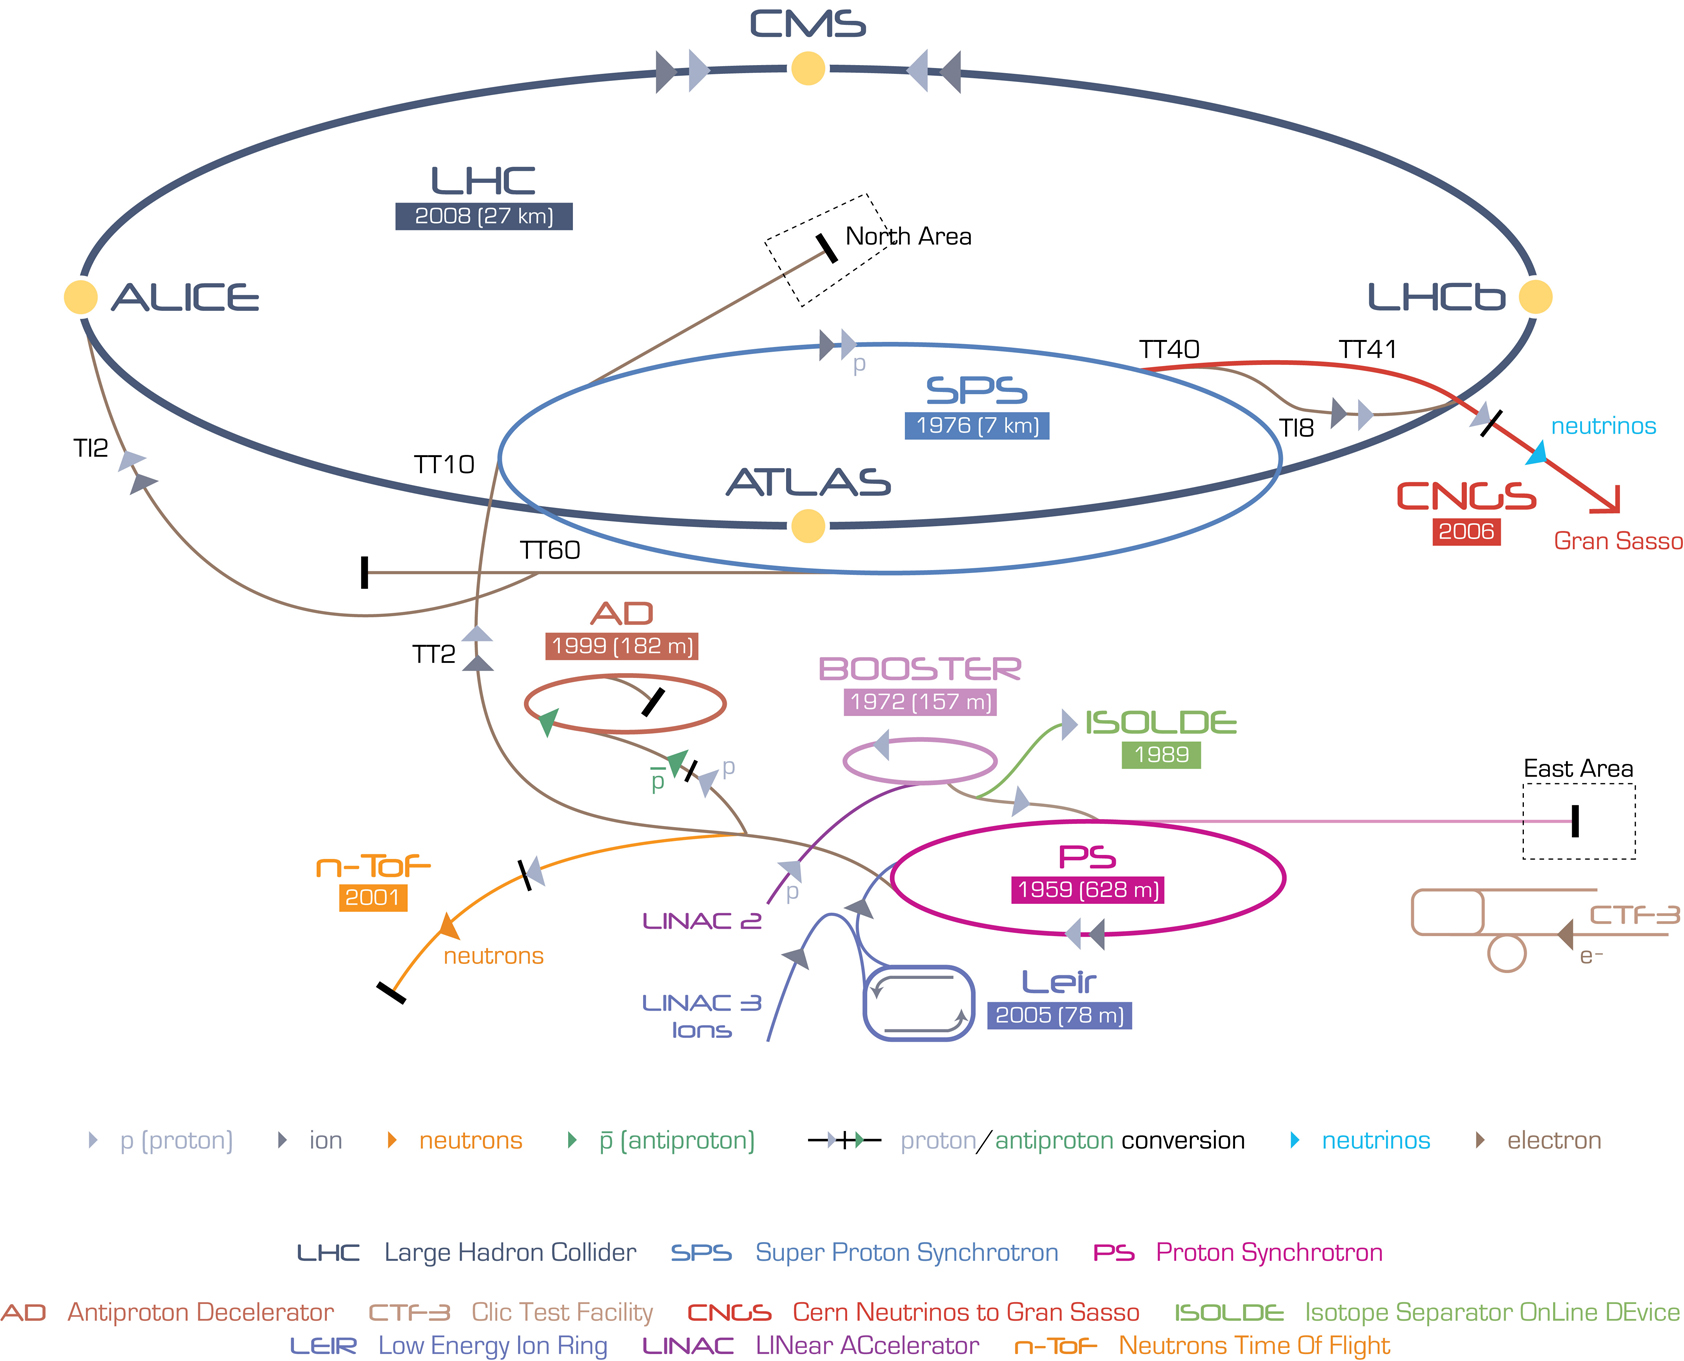
\includegraphics[scale=0.5, angle=0]{figures/Cern-Accelerator-Complex}
    \caption{The full complex of accelerators that dump protons into the LHC
    and other CERN experiments. Protons, which are stripped from hydrogen atoms,
    are accelerated to 99.9\% of the speed of light by passing through a series
    of accelerators: LINAC2, PSB, PS, SPS, and finally the LHC itself.}
  \label{fig:accelerator}
\end{figure}

Particle accelerator performance is characterize by two important quantities:
its center-of-mass energy and luminosity.
The center-of-mass energy of the colliding particles dictates what can
be produced in the collisions.
Larger values are necessary
to produce more massive particles because of conservation of energy and momentum. 
The LHC is designed to collide particles
at a center-of-mass energy of 7 TeV in 2011 and 8 TeV in 2012. This means
that each proton was accelerated to an energy of 3.5 and 4 TeV by the LHC
accelerator complex in 2011 and 2012 respectively. 
In addition to producing high energy collisions,
the LHC must also provide enough collisions to produce rare decay processes,
such as \HToZg.
The event rate $R$ for a physics process with a cross-section $\sigma$
is proportional to the collider's instantaneous luminosity $L$: $R = L\sigma$. 
The luminosity
is characterize by a few important properties of the accelerator:
\[
    L = \frac{k n^2 f}{4\pi \sigma_x \sigma_y}
\]
where $k$ is the number of proton bunches in the proton beam, 
$n$ is the number of protons per
bunch, $f$ is the revolution frequency, and $\sigma_x\sigma_y$ is the
beam size at the collision point. The value of these parameters at the
LHC are given in \refT{tab:lhcparameters}. In addition to being the most
energetic accelerator, the LHC also has the highest luminosity of any particle
collider with an instantaneous luminosity of roughly $10^{34}$ \cm{-2} \sec{-1}.

It should be noted that often what is of interest is not the instantaneous luminosity,
$L$, and the corresponding  event rate $R$, but rather the total number
of events produced of a physics process, i.e. $R \times ~\mathrm{time}$. Therefore,
one is interested in the integrated luminosity defined as 
$\mathcal{L} = \int L dt$, so that $N = \mathcal{L}\sigma$ where
$N$ is the number of events produced of a given process with cross-section $\sigma$.
The integrated luminosity used in this measurement was 4.5 (20.7) \fb in 2011 (2012).

\begin{table}[htbp]
  \begin{center}
    \begin{tabular}{cc}
    \hline\hline
    parameter & value  \\
    \hline
    $k$ &  $1.15 \times 10^{11}$ \\
    $n$ & 2808 \\
    $f$ & 11.25 Hz \\
    $\sigma_x\sigma_y$ &  16 $\mu$m\\
    \hline\hline
    \end{tabular}
    \caption{Parameters characterizing the LHC's luminosity. The integrated luminosity
    used in this measurement was 4.6 (20.7) \fb in 2011 (2012) \cite{LHCdesign}.}
    \label{tab:lhcparameters}
  \end{center}
\end{table}

The operation of the LHC is based on a series of accelerators that get the
proton bunches to the desired center-of-mass energy. Protons are obtained by
stripping hydrogen atoms of their single electron. These protons are then passed into
the LINear ACcelerator 2 or LINAC 2, which is the purple line in the bottom middle
of \refF{fig:accelerator}. The LINAC 2 accelerates these protons to an energy of
50 MeV, or 31.4\% of the speed of light. Then the protons are diverted into the
first circular accelerator, the Booster (denoted as BOOSTER
in Fig. \ref{fig:accelerator}). As well as accelerating protons up to 1.4 GeV,
the booster uses a sequence of quadrupole magnets to squeeze the bunches down 
so that they have a smaller cross-section. Aftward the protons are inserted
into the Proton Synchrotron (PS), which accelerates these protons to an energy
of 25 GeV at a velocity of 99.93\% the speed of light. The PS also uses 
radiofrequency pulses to chop the bunches into smaller sections, which can
be diverted to the various experiments around the CERN accelerator complex.
Then the PS Booster
injects the protons into the Super Proton Synchrotron (SPS) -- the 7 km light blue
ring in the figure. Here protons are accelerated to an energy of 450 GeV,
with a velocity of 99.9998\% the speed of light. These protons finally enter
the LHC ring, which increases the proton energy to 3.5 (4.0) TeV. The result
is a proton beam that collides at 7 (8) TeV in 2011 (2012).

There are six particle detectors located at the LHC designed
to identify the various particles produced during the collisions. TOTEM and LHCf
are designed to measure various scattering cross-sections, diffractive processes, 
and cosmic ray physics. The ALICE detector specializes in detecting the products
of heavy ion collisions in
order to study the quark-gluon plasma of the early universe. ATLAS and CMS 
are general purpose detectors designed to detect a large spectrum of particles
with a goal of finding signs of new physics. The measurement presented in this
paper uses data collected by the ATLAS detector.

\subsection{The ATLAS detector}
\label{subsec:atlas}

The ATLAS detector~\cite{Aad:2008zzm} is a multi-purpose particle physics detector
with approximate forward-backward symmetric cylindrical geometry. The detector
is 25 m in height, 44 m in length, and weights approximately 7000 tonnes. 
Since most particles of interest produced at the LHC are unstable
and decay before they can reach the detector, the ATLAS detector
was designed to detect and distinguish stable particles such as photons,
electrons, and protons. 
The kinematics of the unstable particles
are then calculated from the kinematics of their stable decay products
using conservation of energy and momentum.  In particular, the ATLAS
detector must be able to measure the
number of stable particles that result from the collision, the topology
of the event i.e. the particle's tracks\footnote{The trajectory of a charged
particle through the magnetic field of the detector is reffered to as a track.}, and 
the momentum, energy and identity of these particles.
A single detector cannot measure
all of these properties; therefore, the ATLAS detector consists of various
sub-detectors whose roles fall within two broad categories:
tracking detectors that measure the position of a charged particle with
minimal disturbance, and calorimeters that measure the energy of a particle
by total absorption. The ATLAS detector consists of
an inner tracking detector, an electromagnetic calorimeter, a hadronic calorimeter,
and a muon spectrometer. An artist's rendition of the ATLAS detector is 
displayed in \refF{fig:atlas}.
 
\begin{figure}[!hbpt]
  \centering
  \includegraphics[scale=0.5, angle=0]{figures/atlas}
  \caption{Cut-away view of the ATLAS detector. The dimensions of the detector
  are 25 m in height and 44 m in length. The overall weight of the detector
  is approximately 7000 tonnes.}
  \label{fig:atlas}
\end{figure}

The inner tracking detector (ID) lies closest to the beam pipe and reconstructs
the path of charged particles with the information provided by a 2 T solenoidal
magnetic field. In addition, the inner detector provides momentum
and decay vertex measurements and electron identification. A more in depth
description of the inner tracking system is provided in \refS{subsubsec:id}.
The electromagnetic calorimeter (EM calorimeter) surrounds the inner detector
and measures the energy of light particles that interact electromagnetically such 
as electrons and photons. The hadronic calorimeter encircles the EM calorimeter
and is responsible for measuring the energy of composite hadrons such as protons
and neutrons. The operating principles as well as the geometric details of
the calorimeter system are presented in \refS{subsubsec:calo}. The calorimeter
is surrounded by the muon spectrometer. The muon spectrometer measures the tracks
of the charged muons, which are massive enough to pass through the inner parts
of the detector. The muon spectrometer is described in \refS{subsubsec:muonspec}.

A more complete description of ATLAS splits the detector
into a barrel part, where the detector layers
are positioned on cylindrical surfaces around the beam axis, and two end-cap parts,
where the detector layers are positioned in planes of constant $z$ perpendicular
to the beam pipe. In addition, the calorimeter consists of a forward 
and backward part, extending up to a pseudorapidity\footnote{For a description
of the coordinate system employed at ATLAS see \refS{subsubsec:kinematics}.} 
of $|\eta| < 4.9$. The dimensions of the various components of the ATLAS detector
are displayed in \refT{tab:atlasdim}.

\begin{table}[htbp]
  \begin{center}
    \begin{tabular}{|l|ccc|}
    \hline
    Component & radius [m] & length [m] & $\eta$ coverage \\
    \hline
    barrel muon spectrometer &  11 & 26 & $|\eta| < 1.4$ \\
    end-cap muon spectrometer & 11 & 2.8 & $1.1 < |\eta| < 2.8$ \\
    \hline
    barrel hadronic calorimeter & 4.25 & 12.2 & $|\eta| < 1.0$ \\
    end-cap hadronic calorimeter & 2.25 & 2.25 & $1.5 < |\eta| < 3.2$ \\
    \hline
    barrel em-calorimeter & 2.25 & 6.42 & $|\eta| < 1.4$ \\
    end-cap em-calorimeter & 2.25 & 0.63 & $1.4 < |\eta| < 3.2$ \\
    forward/backward calorimeter & N/A & N/A & $3.1 < |\eta| < 4.9$ \\
    \hline
    barrel + end-cap inner detector & 1.15 & 6.8 & $|\eta| < 2.5$ \\
    \hline
    \end{tabular}
    \caption{Dimensions of the ATLAS sub-detectors.}
    \label{tab:atlasdim}
  \end{center}
\end{table}

\subsubsection{Kinematic quantities at ATLAS}
\label{subsubsec:kinematics}

The geometry of the ATLAS detector is defined
by a right-handed coordinate system with its origin at the point of
the proton-proton collision (PC) located at the center of the detector 
and the $z$-axis along the beam pipe. 
The $x$-axis points from the PC to the center of the LHC 
ring, and the $y$-axis points upward. The $x$ and $y$ axes define
a plane perpendicular to the beam axis known as the transverse plane with
its origin on the beam pipe.

In addition to the rectangular coordinate system previously described,
cylindrical coordinates ($r, \phi$) are
used in the transverse plane, $\phi$ being the azimuthal angle around the
beam pipe. The full 3D geometry is then defined if a third coordinate is specified.
A quantity known as the pseudorapidty is used as the third coordinate, 
which is defined in terms of the 
polar angle $\theta$ as $\eta = -\ln \tan(\theta/2)$, e.g $\theta = 45\degr$
corresponds to $|\eta| = 0.9$. The reason for the use of $\eta$ as opposed
the $\theta$ is because $\eta$ is invariant with respect to longitudinal boosts. This
is important because in hadron collisions one is actually colliding the
constituent quarks and gluons, so that the net longitudinal momentum of the two
colliding partons will vary from collision to collision. Therefore, the laboratory
frame and the parton center of mass frame do not coincide. Instead the parton
center of mass frame is boosted along the beam axis. Thus a distribution
uniform in $\theta$ in the center of mass frame of the partons will not
be uniform in the laboratory frame. However, because $\eta$ is invariant
under longitudinal boosts these two distributions will coincide if $\eta$
is chosen as the third coordinate.

A few other quantities of interest that are invariant under longitudinal boosts
are a particle's transverse momentum $p_T$ and the separation in $\eta-\phi$
space deemed $\Delta R$. The transverse momentum $p_T$ is defined as the 
amount of a particle's momentum that is located in the plane perpendicular 
to the beam pipe (the $x$-$y$ plane). The distance $\Delta R$ 
is defined as $\Delta R = \sqrt{(\Delta \eta)^2 + (\Delta \phi)^2}$.

A kinematic observable that is very effective at discovering particle's at
ATLAS is known as the invariant mass. Consider the Higgs decay process
searched for in this paper: \HTollg where the $Z$ decays into two leptons.
The dilepton invariant mass $m_{\ell\ell}$ is
\[
    m^2_{\ell\ell} = (p_1 + p_2)^2
\]
where $p_1$ and $p_2$ are the four-momenta of the leptons $\ell^+$ and $\ell^-$.
Then
\[
    m_{\ell\ell} = \sqrt{(p_1 + p_2)^2} = \sqrt{(E_1 + E_2)^2 - (\mathbf{p_1} + \mathbf{p_2})^2}.
\]
The relationship of $m_{\ell\ell}$ with the mass $m_Z$ of the Z boson is that a
distribution of $m_{\ell\ell}$ will peak at $m_{Z}$. The concept of invariant
mass can be generalized to a multi-body system such as \HTollg as follows:
\[
    m_{\ell\ell\gamma} = \sqrt{(p_{\ell_1} + p_{\ell_2} + p_{\gamma})^2} =
    \sqrt{(E_{\ell_1} + E_{\ell_2} + E_{\gamma})^2 - (\mathbf{p}_{\ell_1} + 
    \mathbf{p}_{\ell_2} + \mathbf{p}_{\gamma})^2}. 
\]
The distributions of $m_{\ell\ell\gamma}$ and $m_{\ell\ell}$ are the primary
observables used to search for the Higgs boson in this analysis.

\subsubsection{Particle identification at ATLAS}
\label{subsubsec:particleid}
The ATLAS detector is designed so that the various particles produced in
proton-proton collisions leave different signatures in the detector. This
allows for a way to easily distinguish between the particles.
The interactions
of the different particle types with the detector are displayed in 
\refF{fig:particleid}. Photons are uncharged and leave no track in
the inner detector. Therefore, photons are characterized by large energy 
deposits in the electromagnetic calorimeter. Electrons are light charged particles
that interact with the tracking system and deposit their energy into the 
EM calorimeter. Just like the electron, hadrons such as protons and pions 
are charged particles that interact with the inner detector; however, their
large mass causes them to penetrate further into the detector and deposit
their energy into the hadronic calorimeter. Composite neutral particles
like the neutron do not interact with the inner detector; however, they
are detected by the electromagnetic and hadronic calorimeters. Muons
pass through the whole detector and are charged. Thus, they will leave a
track in both the inner detector and the muon spectrometer. Finally,
massless neutrinos which interact only through weak interactions
pass through ATLAS undetected
and are inferred through conservation of energy and momentum.

\begin{figure}[!hbpt]
  \centering
  \includegraphics[scale=0.4, angle=0]{figures/particle-tracks}
 % \begin{subfigure}[b]{0.45\textwidth}
 % \centering
 %     \includegraphics[scale=0.4, angle=0]{figures/particle-signatures}
 %     \caption{}
 %     \label{fig:particleenergy}
 % \end{subfigure}
  \caption{The components the make up the ATLAS detector. Each particle type
  has its own signature in the detector. For example, a particle that is
  only detected in the electromagnetic calorimeter is likely to be a photon.
  }
  \label{fig:particleid}
\end{figure}



% Before delving into the specifics of each component of the ATLAS detector,
% a brief overview of the physical processes responsible for particle detection
% is necessary. Particles are detected through their interactions with matter. As
% such the way in which particles are detected can be broken up into two categories:
% charged and uncharged particle detection. The main processes that lead
% to the detection of charged particles are energy loss through ionization, 
% bremsstrahlung, and hadronic interactions. The process of ionization 
% occurs when charged particles traverse a material and lose energy through
% collisions with atomic electrons, leaving these electrons free from the atom,
% i.e. ionized. This deceleration then leads to emission of a show of photons
% known as bremsstrahlung. The combination of ionization and bremsstrahlung
% is behind the basic operation of the electromagnetic calorimeter.

\subsubsection{The inner detector}
\label{subsubsec:id}
The inner detector surrounds the beam pipe and provides track reconstruction,
momentum information, and both primary and secondary vertex measurements for
charged tracks above a nominal $p_{T}$ threshold of 0.5 GeV and within
a pseudorapidity range of $|\eta| < 2.5$ ($\theta < 10^o$). ATLAS's ID also provides electron
identification over $|\eta| < 2.0$ and 
a range of energies between 0.5 GeV and 150 GeV. The basic
operating principle of the inner detector is to track charged particles
via the ionization of the medium in such a way that the particles lose very
little energy. 

An important ability of the inner detector is to provide a measurement of
a particle's momentum and charge. The whole inner detector is immersed in a 2 T
magnetic field produced by a solenoidal superconducting magnet that radially
surrounds the whole inner detector. The magnetic field produced by the
solenoid is parallel to the beamline, while the particle trajectories are
approximately radial. This means that $\mathbf{v} \times \mathbf{B}$ is proportional
to $\mathbf{\hat r} \times \mathbf{\hat z} = -\mathbf{\hat \phi}$ and
charged particles are deflected tangentially
\footnote{Recall the magnetic
component of the Lorentz force is $\mathbf{F} = q(\mathbf{v} \times \mathbf{B}$).}.
Using hits in all three sub-detectors, a
track of the flight path of a charged particle can be reconstructed. The
curvature of the track is then used to determine the particle's
momentum with the familiar relationship $|p| = \frac{q B}{R}$
where $q$ is the particles charge, $B$ is the strength of the magnetic field, and 
$R$ is the radius of the particle's track. The required momentum resolution
in the inner detector is $\sigma_{p_T}/p_T = 0.05\% p_T \bigoplus 1\%$
\cite{Innerdesign}.

\begin{figure}[!hbpt]
  \centering
  \begin{subfigure}[b]{0.45\textwidth}
      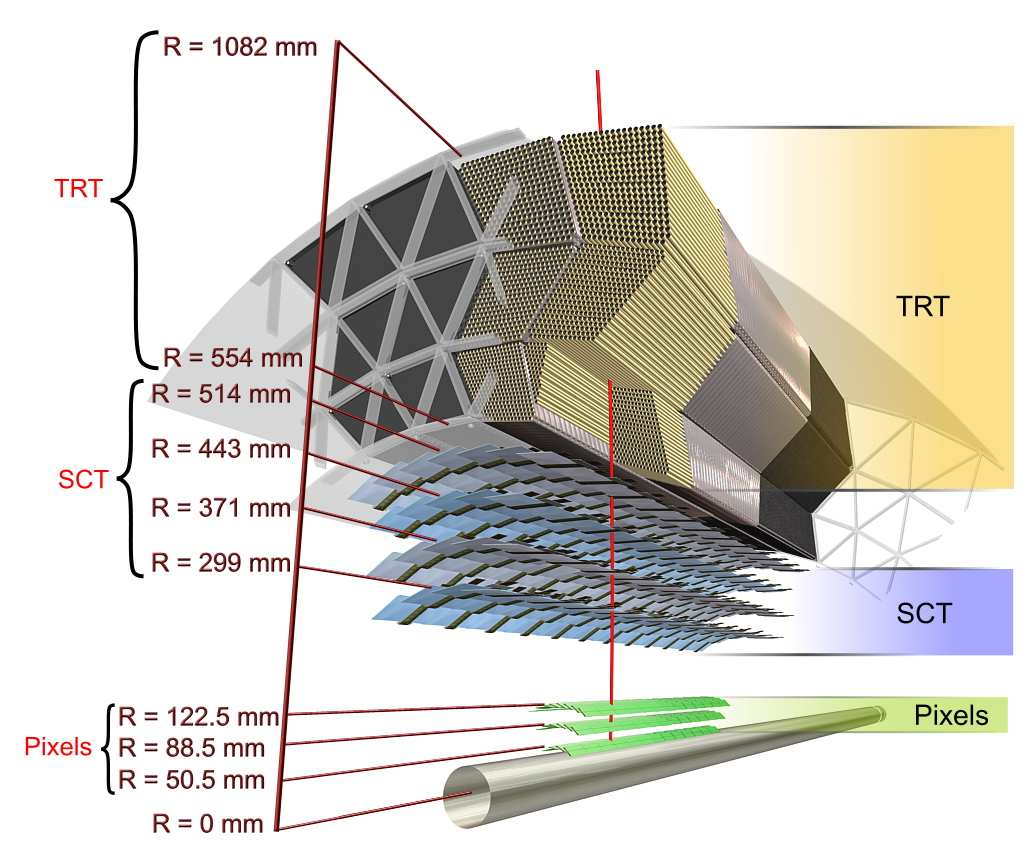
\includegraphics[scale=0.5, angle=0]{figures/id_perspective_layout}
      \caption{}
      \label{fig:idperspective}
  \end{subfigure}
  \quad
  \begin{subfigure}[b]{0.45\textwidth}
  \centering
    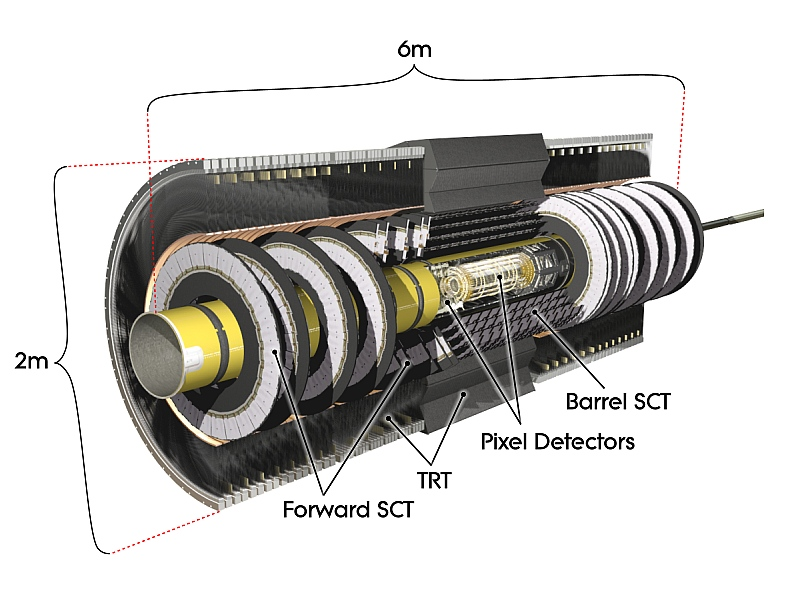
\includegraphics[scale=0.3, angle=0]{figures/Inner_detector}
    \caption{}
    \label{fig:id}
  \end{subfigure}
  \caption{Left-side:
  a cross-sectional view of the inner detector displaying the three tracking
  systems that make it up. Right-side: A complete three-dimensional view
  of the ATLAS inner detector.}
  \label{fig:innerdetector}
\end{figure}

The inner detector is comprised of three tracking systems: pixels,
the silicon central tracker (SCT), and the transition radiation tracker (TRT).
The configuration of these three trackers is displayed in \refF{fig:innerdetector}.
The three trackers operate independently from one another, but the information
is combined to form a complete track of a particle as it makes its way
through the inner detector. The spatial resolution and coverage of the inner detector
sub-systems is displayed in \refT{tab:spaceres}.

\begin{table}[htbp]
  \begin{center}
    \caption{Spatial resolutions and $\eta$-coverage of the sub-detectors
    that make up the ATLAS inner detector \cite{Aad:2008zzm}.}
    \label{tab:spaceres}
    \begin{tabular}{|ll|cc|}
    \hline
    Sub-Detector & Position & Resolution [$\mu$m] & $\eta$ Coverage \\
    \hline
    \textbf{Pixel} & 1 removable barrel layer & $R\phi = 10$, $z = 115$ & $\pm 2.5$ \\
     & 2 barrel layers & $R\phi = 10$, $z = 115$ & $\pm1.7$ \\
     & 4 end-cap disks on each side & $R\phi = 10$, $R = 115$ & 1.7-2.5 \\
    \hline
    \textbf{SCT} & 4 barrel layers & $R\phi = 17$, $z = 580$ &  $\pm 1.4$ \\
     & 9 end-cap wheels on each side & $R\phi = 17$, $z = 580$  & 1.4 - 2.5 \\
    \hline
    \textbf{TRT} & Axial barrel straws & 130 & $\pm 0.7$ \\
     & Radial end-cap straws & 130 & 0.7 - 2.5 \\
    \hline
    \end{tabular}
  \end{center}
\end{table}

\subsubsection*{The pixel detector}
The pixel detector, which sits as close to the interaction point as possible,
provides high precision measurements of a particle's track. The system
consists of 80 million pixels,
each of which is $50 \times 400\mu\mathrm{m}^2$ in dimension. Each charged
particle track transverses three pixel layers, which provides three precision
measurements. The system consists of three barrels at average radii of roughly
5 cm, 9 cm, and 12 cm, 
as well as three disks on each side, between radii of 9 and 15 cm.
The thickness of each layer is about 2.5\% of a radiation length of
nominal incidence.

The millions of pixels that comprise the pixel detector are made of
doped silicon, which acts as a diode when properly biased. These
pixels have a voltage across them to produce a wide depletion region across
the existing p-n junction. This large reverse bias means that no current
will flow through the electronics unless the diode breaks down. However,
when charged particles traverse the bulk silicon, they produce electron-hole pairs
through ionization of the semi-conductor's atoms. This current is then readout
and used to precisely locate the position of the particle. The resolution of
the pixel detector in the $R-\phi$ and $z$ directions 
are displayed in \refT{tab:spaceres}. Note that the resolutions
quoted are typical values and the actual resolution depends on $|\eta|$.

An important 
ability of the pixel detector is to determine the resolution associated with
the measurement of the impact parameter associated with secondary vertices
(decay vertices that occur right after the initial proton-proton collision). 
The minimum distance from the primary vertex to the secondary vertex is called
the impact parameter and it can be broken up into a component in the transverse
plane ($d_0$) and another component along the $z$-axis ($z_0$). A high resolution
of the impact parameter enables identification of secondary vertices
associated with very short-lived particles such as 
b-quarks and $\tau$-leptons. This allows for
better signal to background resolution for important process such as
$H \to b\bar b$ and $t \to W b$. In terms of
the polar angle $\theta$ and the particle's transverse momentum, 
The resolution for $d_o$ is
$\sigma(d_o) = 11 \bigoplus 60/p_T \sqrt{sin\theta}$ and the resolution in $z_o$
is $\sigma(z_o) = 70 \bigoplus 100/p_T \sqrt{sin^3\theta}$ in $\mu$m 
\cite{Aad:2008zzm}.

\subsubsection*{The semiconductor tracker}
At an intermediate radial range the Semiconductor Tracker (SCT) system contributes
to the measurement of momentum, impact parameter, and vertex position.
The SCT operates on the same principles as the pixel
detector; however, narrow strips of silicon $6.36 \times 6.40 \, \text{cm}^2$
in area are used instead of more precise silicon pixels. 
This allows measurement of only one coordinate (either $\phi$ or $z$), so the
SCT uses two orthogonally oriented strips glued back to back to measure both
$\phi$ and $z$. The four barrel layers are located at radii of roughly 3 cm,
3.71 cm, 4.43 cm, and 5.14 cm. This allows for four precision measurements of
a track's $R$, $\phi$, and $z$ coordinates. 
The spatial resolution of the SCT system is documented in \refT{tab:spaceres}.
Two tracks can be distinguished if they are separated by more than 200 $\mu$m.

\subsubsection*{The transition radiation tracker}
The transition radiation tracker (TRT) surrounds both the pixel and SCT detectors.
The TRT is a straw tracker made of roughly 60 layers of 
Polymide drift tubes (straws) of 4 mm diameter and filled with a combination
of Xenon, CO$_2$, and O$_2$ gas. 
The barrel contains about 50000 straws, and the end-caps contain 320000 radial straws.
When a charged particle transverses the drift tubes, the gas is ionized within
the straw. A voltage is applied to the wall of the straw and the central wire in
such a way that the negative free electrons resulting from the ionized gas
will drift to the central wire. The electron's drift velocity is known. Therfore,
the distance from the center of the straw to the flight path of the charged
particle can be determined using the timing between the arrival of the first
and last ionized electron. This process is outlined in \refF{fig:trt}. The
TRT only measures the position of a particle in the $\phi$ direction with
a resolution of 130 $\mu$m.

\begin{figure}[!hbpt]
  \centering
  \includegraphics[scale=0.4, angle=0]{figures/trtschematic}
  \caption{Cross-section of a bundle of TRT straw tubes.}
  \label{fig:trt}
\end{figure}

As well as providing spatial tracking, the TRT is designed to identify
electrons. The space between the straws is filled with a foam that has
a different index of refraction than the Xenon gas within the straws. When
ultra-relativistic particles\footnote{Particles with $\gamma = (1 - \beta^2)^{\frac{1}{2}} \approx 2000$.} cross the boundaries of these materials, they produce
transition radiation. This additional radiation will produce a high threshold
signature in the straw. Along with the energy measurement provided by the
calorimeter system, the presence of transition radiation can help identify
the particle as an electron (via $E = \gamma m c^2$).
 
% \begin{figure}[!hbpt]
%   \centering
%   \includegraphics[scale=0.4, angle=0]{figures/impactparameter}
%   \caption{Cross-section of a bundle of TRT straw tubes.}
%   \label{fig:trt}
% \end{figure}

\subsubsection{The calorimeter}
\label{subsubsec:calo}
The ATLAS calorimeter system is placed between the inner detector and the muon
spectrometer. The primary purpose of the calorimeters is to measure the energy
of both charged and neutral particles such as electrons, photons, and jets, 
and to determine the missing transverse energy. 
In addition, the calorimeters provide crude position measurements
as well as particle identification.

Calorimetry operates through the measurement of an incident particle's energy
by total absorption, where a fraction of the total energy is transformed
into a measurably quantity, i.e. charge or light. In practice,
each calorimeter is composed of metal sheets known as absorbers sandwiched 
between a detection medium. Particles interact with the absorbers transforming
the incident energy into a `shower' of secondary particles that are detected
in the detection medium. In a crude sense, the total number of particles
produced in these showers is proportional to the energy of the incident particle.
Thus, a calorimeter is a device designed to count secondary particles 
produced in these interactions.

\begin{figure}[!hbpt]
  \centering
  \includegraphics[scale=0.5, angle=0]{figures/calorimeter}
  \caption{Cut-away view of the ATLAS calorimeter system.}
  \label{fig:cal}
\end{figure}

The calorimeter system covers the range $|\eta| < 4.9$ and is composed of an
electromagnetic and hadronic calorimeter. The EM calorimeter is designed for
precision measurements of electrons and photons, while the hadronic calorimeter is
responsible for providing accurate measurements of jet energy and the reconstruction
of missing transverse energy $\slashed{E}_T$. The calorimeter was also designed
to contain the electromagnetic and hadronic showers so that they do not
make it through to the muon systems. Thus, the total thickness of the EM 
calorimeter is $> 22$ radiation lengths ($X_0$) in the barrel and $> 24\,X_0$
in the end-caps.
An overview of the ATLAS calorimeter system is displayed in \refF{fig:cal}.

\subsubsection*{Electromagnetic calorimeter}
The EM calorimeter consists of lead absorbers and liquid argon (lAr) sensing
elements, which provide optimized energy and position resolution for electrons
and photons within a pseudorapidity range of $|\eta| < 3.2$. The calorimeter
itself is split into a barrel part ($|\eta| < 1.475$) and two end-cap components
($1.375 < |\eta| < 3.2$). The EM calorimeter occupies a cylinder of 13.30 m in length
with an outer radius of 2.25 m.  Within this cylinder the calorimeter consists
of an accordion-shaped network of 1.5 mm thick lead plates separated 
by 4 mm of liquid argon. The accordion geometry provides complete $\phi$ symmetry
without azimuthal cracks.

\begin{figure}[!hbpt]
  \centering
  \includegraphics[scale=0.5, angle=0]{figures/emcal}
  \caption{A cross-section of the EM calorimeter.}
  \label{fig:emcal}
\end{figure}

The operation of the EM calorimeter is based on the detection of electron-positron
pairs and photons that arise from bremsstrahlung and pair-production when high
energy electrons and photons hit the lead absorbers. When these charged
secondary particles traverse the liquid argon, they ionize the argon.
These ions and free electrons then drift to external electric terminals where
they are sensed as a current. Two phenomena contribute to the reconstruction
of the incident particle's energy: 1) the more energetic the particle, then
the more showers it will produce causing more ionization of the liquid argon,
2) highly energetic particles will penetrate deeper into the calorimeter.
Both phenomena are used to measure the total energy of the incident particle.
The required energy resolution in the EM calorimeter is 
$\sigma_E/E = 10\% / \sqrt{E} \bigoplus 0.7\%$ \cite{Lardesign}.

In addition to energy measurements, the EM calorimeter provides spatial
measurements. The region $|\eta| < 2.5$ is devoted to the 
performance of these precision measurements.
In this region the calorimeter is segmented into three sections. The first
layer acts as a pre-shower detector. This layer has a constant thickness of
6 $X_0$ as a function of $\eta$. It has a resolution of $\Delta\eta \times
\Delta\phi = 0.003 \times 0.1$, and provides a precise measurement of
the pseudorapidity. This high granularity also enhances the ability to distinguish
between photons, pions, and electrons. The second layer is segmented into towers
of size $\Delta \eta \times \Delta\phi = 0.025 \times 0.025$. The first
and second layers have a total thickness of about 24 radiation lengths which
decrease as a function of $\eta$. The last layer has a resolution of 
$\Delta\eta \times \Delta\phi = 0.05 \times 0.025$ and a thickness of
2 $X_0$, which increases as a function of $\eta$. A summary of the EM 
calorimeter's resolution is given in \refF{fig:emcal}.

\subsubsection*{Hadronic calorimeter}
The hadronic calorimeter encircles the electromagnetic calorimeter and
provides measurements of jet energy and missing transverse energy. The hadronic
calorimeter is also responsible for containing hadron showers induced by
protons, neutrons, pions, and kaons so that they do not enter the muon spectrometer.
As such, the hadronic calorimeter has a thickness of 11 interaction
lengths, which reduces the hadronic leakage to well below the rates for muons.
The hadronic calorimeter consists of three sub-detectors: the tile 
calorimeter, the hadronic end-cap calorimeter (HEC) and the forward hadron
calorimeter (FCal). A summary of the energy resolution and $\eta$ coverage
of the hadronic calorimeter is given in \refT{tab:calres}.

\begin{table}[htbp]
  \begin{center}
    \caption{The resolution and $\eta$ coverage of the ATLAS hadronic calorimeter.}
    \label{tab:calres}
    \begin{tabular}{|l|c|c|}
    \hline
    Detector component & Required resolution & $\eta$ coverage  \\
    \hline
    Barrel and end-cap & $\sigma_E / E = 50\% / \sqrt{E} \bigoplus 3\%$ & $\pm3.2$ \\
    forward & $\sigma_E / E = 100\% / \sqrt{E} \bigoplus 10\%$ & $3.1 < |\eta| < 4.9$ \\
    \hline
    \end{tabular}
  \end{center}
\end{table}

The tile calorimeter covers an $\eta$ range $|\eta| < 1.0$ and its two
extended barrels range between $0.8 < |\eta| < 1.7$. The calorimeter uses steel
as the absorber and scintillating tiles as the active material. When
incident hadrons -- components of particle jets -- interact with the steel
plates via the electromagnetic and strong force, they produce a shower of hadrons,
electron-positron pairs, and photons. As these hadrons pass through the scintillating 
tiles, they cause the tiles to produce light that is amplified by a photomultiplier
tube and then detected. The energy of the initial hadron effects the detection
system in two ways: more energetic hadrons produce more showers leading to more
light produced in the scintillator, and their showers also penetrate further
into the calorimeter. Both phenomena are used by the barrel tile calorimeter
to measure the initial hadron's energy. The tile calorimeter consists of
three consecutive layers with a granularity of $\Delta\eta \times \Delta\phi =
0.1 \times 0.1$ in the first two layers and $\Delta\eta \times \Delta\phi =
0.2 \times 0.1$ in the third layer. It should be noted that hadrons can initiate
showers in the electromagnetic calorimeter, and the signals from both electromagnetic
and hadronic calorimeters must be combined in order to obtain the full energy of the
hadron.

The HEC and FCAL extend the hadronic calorimeter to an $|\eta|$ range of 4.9. 
Because of the intense radiation emitted by the proton-proton collisions at large
pseudorapidities, the scintillating tiles used in the tile calorimeter are replaced
with the liquid argon detectors used in the EM calorimeter. The reason being that
the scintilating tiles would be damaged by the excessive radiation dose.
The only compositional difference between 
these calorimeters and the EM calorimeter is that the HEC uses copper absorbers
and the FCAL uses copper and tungsten. These materials are used instead of lead
because they interact better with the incident hadrons.

\subsubsection{The muon spectrometer}
\label{subsubsec:muonspec}

The only particles that make it through the calorimeters are muons and neutrinos
\footnote{Neutrinos are not detected by the ATLAS detector and are 
inferred from the missing transverse energy measured in the calorimeters.},
so various ionization tracking chambers comprise 
the muon spectrometer to measure the muon's kinematics.
The muon spectrometer consists
of two precision tracking detectors: the Monitored Drift Tubes (MDT) and the
Cathode Strip Chamber (CSC). In addition to the tracking chambers, which
determine the sign of the muon's charge and perform 
high-precision measurements of the muon's momentum, the muon spectrometer 
contains triggering chambers. These are the Resistive Plate Chamber (RPC)
and the Thin Gap Chamber (TGC). The set-up of the muon spectrometer is displayed
in \refF{fig:muonspec}.

\begin{figure}[!hbpt]
  \centering
  \includegraphics[scale=0.4, angle=0]{figures/muonspec}
  \caption{Cut-away view of the ATLAS muon spectrometer.}
  \label{fig:muonspec}
\end{figure}

The hits recorded by the muon spectrometer sub-detectors are reconstructed into
the track of muon's flight path. The muon is then matched to an inner detector
track by the ATLAS reconstruction software MuID and STACO. This forms one complete
muon track that traverses the whole ATLAS detector.

\subsubsection*{Toroid magnets}
Eight superconducting toroid magnets in the barrel and another eight 
superconducting toroid magnets in the end-caps create a magnetic field that
permeates throughout the muon spectrometer. Within the region $|\eta| < 1.4$
a 0.5 T magnetic field is provided by the barrel toroid.  A region between
$1.4 < |\eta| < 1.6$ represents the transition region where the magnetic deflection
is due to both the barrel and end-cap magnets. Finally, a 1 T magnetic field
is produced by the toroid magnetics in the end-cap region of $1.6 < |\eta| < 2.7$.

The toroidal field is roughly along $\mathbf{\hat \phi}$ and is thus
orthogonal to the muon trajectories. In the barrel region the muon trajectories
are mostly radial. Therefore, the deflection is primarily in the
direction of $\mathbf{v} \times \mathbf{B}$ or $\mathbf{\hat r} \times \mathbf{\hat \phi} = \mathbf{\hat z}$, i.e. parallel to the beam pipe.
However, in the end-cap region the muon velocity has a large z component. This
means that $\mathbf{v} \times \mathbf{B}$ has a large radial component, and the
deflection tends to be radial.

Just as in the inner detector, the path of the muon can be reconstructed and
the muon's momentum can be measured by the curvature of its track. Moreover,
the muon tracks can be combined with measurements from the inner detector to 
track the muons over long distance.  This not only provides very precise measurements
of muon momentum, but allows for efficient muon identification by
tagging muons as any energetic particle emerging from the calorimeter whose track 
originates close to the collision point. The momentum resolution of the muon
spectrometer is $\sigma_{p_T}/p_T = 10\%$ at $p_T = 1$ TeV.
Precision measurements of these
track coordinates are provided by the Monitored Drift Tubes and the Cathode
Strip Chambers.

\subsubsection*{Monitored drift tubes}
The Monitored Drift Tubes (MDT) consist of three to eight layers of drift tubes
and covers an $\eta$ range of $|\eta| < 2.7$. However, the inner-most layer of
the MDT only extends to $|\eta| < 2.0$. The cathode strip chambers are installed at
the larger pseudorapidities ($2 < |\eta| < 2.7$), because they are better suited
to deal with the high flux of background particles. The drift tubes that
compose the MDT are aluminum tubes of 30 mm diameter with a central tungsten-rhenium
wire of 50 $\mu$m diameter. The tubes contain a mixture of 93\% argon and
7\% CO$_2$ gas.

The operation of the MDT is similar to the straw tubes of the TRT in the inner
detector. An in depth discussion of these operating principles is given
in \refS{subsubsec:id}. The primary purpose of the MDT is to measure the
coordinates of the muon track in the bending direction, i.e. along the
beam pipe for muons in the barrel. The resolution of the MDT is 80 $\mu$m per
tube.

\subsubsection*{Cathode strip chambers}
At large pseudorapidities the Cathode Strip Chambers (CSC) replace
the MDT since their higher granularity allows them to withstand the large
density of muons in the forward region. The CSC are multi-wire proportional
chambers with wires oriented in the radial direction. The chambers are formed
with strips of cathode capacitor plates on either side and a row of anode
wires sandwiched in between. The cathode strip chambers are filled with a mixture
of 30\% argon, 50\% CO$_2$, and 20\% CF$_4$ gas. As a charged particle passes
through the chamber it will ionize the gas in the chamber, freeing electrons
and positively charged ions. The negatively charged electrons will flow toward the
anode wires and the positive ions drift to the cathode plates. A single muon
may induce an avalanche of electrons and ions that end up on different wires
and strips since the ionization area has some spread. Therefore, the CSC
determines the muon's position by interpolating the induced positive charge on 
3 to 5 adjacent strips. 
The structure and operating principle of the CSC is shown in \refF{fig:csc}.

\begin{figure}[!hbpt]
  \centering
  \begin{subfigure}[b]{0.45\textwidth}
      \includegraphics[scale=0.2, angle=0]{figures/csclayout}
      \caption{}
      \label{fig:csclayout}
  \end{subfigure}
  \quad\quad\quad
  \begin{subfigure}[b]{0.45\textwidth}
  \centering
    \includegraphics[scale=0.3, angle=0]{figures/csccharge}
    \caption{}
    \label{fig:csccharge}
  \end{subfigure}
  \caption{Left: structure of the CSC cells looking down at the wires. 
  Right: superposition of the charge distribution in the perpendicular direction
  over the cathode strips. The distribution must be combined over 3-5 readout strips.}
  \label{fig:csc}
\end{figure}

The wires are arranged in the radial directions in order to measure the $\phi$
coordinate of the muon. On one side, the cathode strips are arranged parallel to 
the wire to complement the measured $\phi$ coordinate of the muon and to reduce noise.
On the other side, the cathode strips are arranged transverse to the wires to measure
the $\eta$ coordinate of the muon. The spatial resolution achieved by the CSC
is $\Delta \eta \times \Delta \phi = 40~\mu\mathrm{m} \times 5~\mathrm{mm}$.
The electron drift time is 30 ns, and the time resolution is 7 ns.

\subsubsection*{Muon triggering system}
The muon triggering system covers the pseudorapidity range $|\eta| < 2.4$  The
triggering chambers are designed with three goals in mind: trigger on muons with 
a transverse momentum greater than a cutoff $p_T^{\text{cut}}$, distinguish
between proton bunch crossings that occur every 25 ns, and to quickly measure the 
muon coordinate in the direction orthogonal to that determined by the 
precision tracking chambers. The triggering system contains three layers of
resistive plate chambers (RPT) in the barrel, and thin gap chambers (TGC) 
in the end-caps.

The resistive plate chambers are gaseous parallel electrode plate (i.e. no wire)
detectors, which provide a spatial and temporal resolution of 1 cm $\times$ 1 ns.
The RPC is formed by two parallel cathode/anode plates kept a distance of 2 mm by
insulating spacers. The chambers contain primarily C$_2$H$_2$F$_4$ with a
small mixture of SF$_6$ to allow operation at relatively low voltages.
The gas is chosen such that the gas sparks when muons pass through. The sparking
allows near instantaneous detection of muons instead of waiting for the electrons
and positive ions to drift to the plates. The RPC permits the trigger to select
high momentum tracks in the range 9-35 GeV (high $p_T$ trigger), while
also providing a low-$p_T$ trigger in the range 6-9 GeV.

The thin gap chamber consists of multiwire proportional chambers similar
in design to the CSC. The TGC provides two functions in the end-cap muon spectrometer:
the muon triggering capability and the determination of the second, azimuthal 
coordinate to complement the measurement of the MDT's in the radial direction.
The TGC covers the $|\eta|$ range between 1.05 and 2.7. However, the TGC
can only trigger up to an $|\eta|$ of 2.4.

\subsection{The triggering system}
The bunch crossing rate for the LHC is $\sim 40$ MHz. At the designed luminosity
$L = 10^{34}$ cm$^{-2}$ s$^{-1}$ the interaction rate is about 1 GHz. However,
due to CPU limitations the rate at which events are selected must be reduced
to $\sim 100$ Hz before permanent storage. This requires a rejection of
a factor of $10^7$ against minimum bias events\footnote{This means that
one tries to be as unbiased as possible in there selection of collisions 
to save to disk. Of course one cannot be truly unbiased and must choose
to remove events based on some criterion. ATLAS measures particle distributions
for events where there is at least one track in a given region of the detector.}.
The problem faced in triggering at the LHC is that the cross-sections for
process of interest are very small, so the selection must be very 
efficient.

The trigger is a collection of hardware and software designed to perform
the selection process which chooses events to be permanently recorded for
off-line analysis. The ATLAS triggering system consists of three level triggers,
each of which refines the decision made during the previous step by applying
additional criteria. The Level 1 (L1) trigger uses information from the
calorimeters and the muon triggering systems to reduce the event rate from
40 MHz to about 75 kHz. Next the Level 2 trigger uses reconstructed electron,
photon, muon, and jet information to reduce the rate to 4 kHz. Finally,
the event filter selects events at a rate of 200 Hz with an event size
of approximately 1.3 Mbyte. This corresponds to about 300 MB/s of data written 
to disk and 3 Pbytes of data stored every year. \refF{fig:trigger} displays 
a diagram of the triggering and data acquisition (DAQ) systems.

\begin{figure}[!hbpt]
  \centering
  \includegraphics[scale=0.4, angle=0]{figures/triggersystem}
  \caption{Flow chart of the ATLAS trigger system.}
  \label{fig:trigger}
\end{figure}
